% methods goes here. 
In this section, we present our \textit{comparison-free},\textit{matrix-free}, \textit{mesh-free} algorithms for performing FEM computations on $kD$ trees. Several state-of-the-art approaches \cite{FernandoDendroGR, Dendro, SundarSampathBiros08, SundarMalhotraBiros13, dealII90, mfem} use a comparison operator induced by a Space Filling Curve (SFC) to sort and partition the nodes of the tree\cite{FernandoSundar16}. The matrix-free FEM computations are widely used in the HPC community\cite{Dendro, mantle, dealII90, mfem}, due to better scalability compared to the matrix-based approaches. Here matrix-free FEM approaches refer to FEM computations without the explicit assembly of matrices,  instead providing a matrix-vector product (\mvec). These are also particularly efficient for non-linear operators, which would require repeated assembly. 
%
For performing matrix assembly or a \mvec\, we need neighborhood data structures such as \textit{element to nodal mapping} or \textit{nodal to nodal mapping}. 
We refer to such data structures % used to perform numerical computations,we refer to
as the mesh (connectivity information).

There are several major drawbacks of comparison- and mesh- based numerical computations on adaptive trees. 
Firstly, since the elements are ordered based on the SFC, it is possible to use binary search to find neighbors among the list of elements. However, for large numbers of elements (as in the case of $4D$), this can result in memory access forcing a cache misses least for the initial few accesses. Secondly, despite the locality of the SFC, neighbors are not contiguous in memory. During an assembly/\mvec\ operation, the separation between neighbours will cause inefficient memory access. More importantly, the use of a mesh causes indirect memory access of the variable (\mintinline{C++}{u[mesh[elem,node]]} instead of \mintinline{C++}{u[node++]}), making it difficult for compilers to prefetch data. 
% The  ordering of the tree leaf nodes is used to perform, binary search operations in order to build the above neighborhood data structures. The binary search operations result in unstructured memory accesses leading to bad memory performances especially the number of search keys increases (see Figure \ref{}). 
%
% The mesh-based FEM computations require indirect memory accesses to the underlying variables defined on the grid \mf{if disable the ability to prefetch the data, in streaming processor architectures} (see Figure). 
%
As the dimensionality $k$ increases, building neighborhood data structures becomes extremely complex, increases storage, and makes the algorithm computationally expensive. The last factor is particularly important for problems requiring frequent mesh-refinements. 

In order to overcome the above challenges we propose a mesh-free \mvec\ that avoids these issues by computing the neighborhood information on the fly, similar to how matrix-free methods work without explicitly storing the matrix entries. We therefore end up with a 
%
\textit{comparison-free, mesh-free, matrix-free} algorithm for performing FEM computations on $kD$ trees. 

\subsection{\tsort: comparison-free SFC based tree partitioning}
\label{subsec:tsort}
Given that we are interested in generating a space-traversal, more so of application specific coordinates or regions, it is efficient to consider this problem as a traversal of the points in the SFC order. Specifically, we construct the tree in a \textit{top-down} fashion, one level at a time, arranging the nodes at a given level based on the recurrence rules for the specific SFC. We call this algorithm \tsort ~(Algorithm~\ref{alg:tsort}). There are two main advantages for this approach: 1). The comparison-free property makes the structure of \tsort~ independent of the SFC being used\cite{FernandoDuplyakinSundar17}. 2). The top-down traversal of the tree in breadth-first fashion, which is performed in the distributed \tsort~, gives us explicit control over the  load-imbalance, which can be tuned as specified in \cite{FernandoSundar16}. All subsequent operations, such as tree construction, enforcing 2:1 balancing, and the \mvec~ operation in FEM computations, are performed using top-down and bottom-up traversals with slight variations of the sequential \tsort~ algorithm. 

\begin{algorithm}[t]
  \caption{\tsort}\label{alg:tsort}
  \footnotesize
  \begin{algorithmic}[1]
    \Require A list of points or regions $W$, the starting level $l_1$ and the ending level $l_2$
    \Ensure $W$ is reordered according to the SFC.
    %\Function{TreeSort($W$, $l_1$, $l_2$)}{}
    \State $counts [] \leftarrow 0$
    \Comment $|counts| = 2^{d}$, 16 for $4D$
    \For{$w \in W$}
    \State increment $counts[child\_num(w)]$
    \EndFor
    % Bucket($W$, $l$) 
    \State $counts [] \leftarrow R_h(counts)$ 
    \Comment Permute counts using SFC ordering
    \State offsets [] $\leftarrow scan(counts)$
    \For{$w \in W$}
    \State $i\leftarrow child\_num(w)$
    \State append $w$ to $W_i$ at offsets$[i]$
    \State increment offset$[i]$
    \EndFor 
    \If{$l_1 > l_2$} 
    \For{$i:=1:2^{d}$}
    \State \tsort ($W_i, l_1-1, l_2$)
    \Comment local sort
    \EndFor 
    \EndIf
    %\EndFunction
    \State \Return $W$
  \end{algorithmic}
\end{algorithm}

\begin{algorithm}[t]
  \caption{\dsort: Distributed \tsort}\label{alg:dsort}
  \footnotesize
  \begin{algorithmic}[1]
    \Require A distributed list of points or regions $W_r$, $\mathit{comm}$, $p$ (w.l.g., assume $p= mk$),
    $p_r$ of current task in $\mathit{comm}$, $tol$ load flexibility, 
    \Ensure globally sorted array $W$
    %\State $split\_count \leftarrow 1$
    \State $counts\_local \leftarrow [\ ], counts\_global \leftarrow [\ ]$    
    \State $s [] \leftarrow \tsort(W_r,l-\log(p),l)$ \Comment initial splitter computation
    
    \While {$|s_r-\frac{rn}{p}|>tol$}     
    \State $counts[] \leftarrow 0$ \Comment $|counts| = 2^{d}$, 16 for 4D
    \For{$w \in W$}
    \State increment $counts[child\_num(w)]$
    \EndFor
    \State $counts\_local [] \leftarrow push(counts)$  
    \State $counts [] \leftarrow R_h(counts)$ 
    \Comment Permute counts using SFC ordering
    \State offsets $[] \leftarrow scan(counts)$
    \For{$w \in W$}
    \State $i\leftarrow child\_num(w)$
    \State append $w$ to $W_i$ at offsets$[i]$
    \State increment offset$[i]$
    \EndFor
    %\State $split\_count \leftarrow 2^{dim}\times split\_count$

    \State $\mathtt{MPI\_ReduceAll}(counts\_local,counts\_global,comm)$
    \State $s[] \leftarrow select(s,counts\_global)$
    \EndWhile
    %	  \State $\mathtt{MPI\_AlltoAllv}$(A,splitters,comm)
    % \Comment optimal splitter computation (with in the given tolerance)	  
    \State $\mathtt{MPI\_AlltoAllv}$(A,splitters,comm)
    \Comment Staged All2all
    \State \tsort$(W_r, 0, l)$ \Comment local sort
    \State \Return $W_r$
  \end{algorithmic}
\end{algorithm}


\begin{figure}
	\begin{tikzpicture}[scale=0.2,every node/.style={scale=0.6}]
	% \draw[gray, very thin] (0,0) grid +(8,8);
	\draw (0,0) rectangle +(8,8);
	\draw[fill=cpu3] (0.5,7.5) circle (0.2);
	\draw[fill=cpu4] (1.5,6.5) circle (0.2);
	\draw[fill=cpu1] (4.5,2.5) circle (0.2);
	\draw[fill=cpu2] (5.5,3.5) circle (0.2);
	\draw[fill=cpu5] (7.5,0.5) circle (0.2);
	
	\begin{scope}[shift={(11,0)}]
	\draw[step=4] (0,0) grid +(8,8);
	\draw[fill=cpu3] (0.5,7.5) circle (0.2);
	\draw[fill=cpu4] (1.5,6.5) circle (0.2);
	\draw[fill=cpu1] (4.5,2.5) circle (0.2);
	\draw[fill=cpu2] (5.5,3.5) circle (0.2);
	\draw[fill=cpu5] (7.5,0.5) circle (0.2);

	\draw [cyan,thick, xshift=0cm] plot [smooth, tension=1] coordinates { (2,2) (6,2) (6,6) (2,6)};
	
	\node at (-1,7.5) {$\mathbf{1}$\textcolor{cpu3}{$\mathbf{1 1}$}};
	\node at (-1,6.5) {$\mathbf{1}$\textcolor{cpu4}{$\mathbf{1 0}$}};
	\node at (-1,3.5) {$\mathbf{0}$\textcolor{cpu2}{$\mathbf{1 1}$}};
	\node at (-1,2.5) {$\mathbf{0}$\textcolor{cpu1}{$\mathbf{1 0}$}};
	\node at (-1,0.5) {$\mathbf{0}$\textcolor{cpu5}{$\mathbf{0 0}$}};
	
	\node[rotate=-90] at (0.5,-1) {$\mathbf{0}$\textcolor{cpu3}{$\mathbf{0 0}$}};
	\node[rotate=-90] at (1.5,-1) {$\mathbf{0}$\textcolor{cpu4}{$\mathbf{0 1}$}};
	\node[rotate=-90] at (5.5,-1) {$\mathbf{1}$\textcolor{cpu2}{$\mathbf{0 1}$}};
	\node[rotate=-90] at (4.5,-1) {$\mathbf{1}$\textcolor{cpu1}{$\mathbf{0 0}$}};
	\node[rotate=-90] at (7.5,-1) {$\mathbf{1}$\textcolor{cpu5}{$\mathbf{1 1}$}};
	\end{scope}
	
	\begin{scope}[shift={(22,0)}]
	\draw[step=4] (0,0) grid +(8,8);
	\draw[step=2] (4,0) grid +(4,4);
	\draw[step=2] (0,4) grid +(4,4);
	\draw[fill=cpu3] (0.5,7.5) circle (0.2);
	\draw[fill=cpu4] (1.5,6.5) circle (0.2);
	\draw[fill=cpu1] (4.5,2.5) circle (0.2);
	\draw[fill=cpu2] (5.5,3.5) circle (0.2);
	\draw[fill=cpu5] (7.5,0.5) circle (0.2);
	
	\node at (-1,7.5) {$\mathbf{11}$\textcolor{cpu3}{$\mathbf{1}$}};
	\node at (-1,6.5) {$\mathbf{11}$\textcolor{cpu4}{$\mathbf{0}$}};
	\node at (-1,3.5) {$\mathbf{01}$\textcolor{cpu2}{$\mathbf{1}$}};
	\node at (-1,2.5) {$\mathbf{01}$\textcolor{cpu1}{$\mathbf{0}$}};
	\node at (-1,0.5) {$\mathbf{00}$\textcolor{cpu5}{$\mathbf{0}$}};
	
	\node[rotate=-90] at (0.5,-1) {$\mathbf{00}$\textcolor{cpu3}{$\mathbf{0}$}};
	\node[rotate=-90] at (1.5,-1) {$\mathbf{00}$\textcolor{cpu4}{$\mathbf{1}$}};
	\node[rotate=-90] at (5.5,-1) {$\mathbf{10}$\textcolor{cpu2}{$\mathbf{1}$}};
	\node[rotate=-90] at (4.5,-1) {$\mathbf{10}$\textcolor{cpu1}{$\mathbf{0}$}};
	\node[rotate=-90] at (7.5,-1) {$\mathbf{11}$\textcolor{cpu5}{$\mathbf{1}$}};
	\draw [cyan,thick, xshift=0cm] plot [smooth, tension=1] coordinates { (2,2) (5,1) (7,1) (7,3) (5,3) (6,6) (3,7) (3,5) (1,5) (1,7)};
	\end{scope}
	
	\begin{scope}[shift={(33,0)}]
	\draw[step=4] (0,0) grid +(8,8);
	\draw[step=2] (4,0) grid +(4,4);
	\draw[step=2] (0,4) grid +(4,4);
	\draw (0,6) grid +(2,2);
	\draw (4,2) grid +(2,2);
	
	\draw[fill=cpu3] (0.5,7.5) circle (0.2);
	\draw[fill=cpu4] (1.5,6.5) circle (0.2);
	\draw[fill=cpu1] (4.5,2.5) circle (0.2);
	\draw[fill=cpu2] (5.5,3.5) circle (0.2);
	\draw[fill=cpu5] (7.5,0.5) circle (0.2);
	
	\node at (-1,7.5) {$\mathbf{111}$};
	\node at (-1,6.5) {$\mathbf{110}$};
	\node at (-1,3.5) {$\mathbf{011}$};
	\node at (-1,2.5) {$\mathbf{010}$};
	\node at (-1,0.5) {$\mathbf{000}$};
	
	\node[rotate=-90] at (0.5,-1) {$\mathbf{000}$};
	\node[rotate=-90] at (1.5,-1) {$\mathbf{001}$};
	\node[rotate=-90] at (5.5,-1) {$\mathbf{101}$};
	\node[rotate=-90] at (4.5,-1) {$\mathbf{100}$};
	\node[rotate=-90] at (7.5,-1) {$\mathbf{111}$};
	\draw [cyan,thick, xshift=0cm] plot [smooth, tension=1] coordinates { (2,2) (5,1) (7,1) (7,3) (5.5,3.5) (5.5,2.5) (4.5,2.5) (4.5,3.5) (6,6) (3,7) (3,5) (1,5) (0.5,6.5) (1.5,6.5) (1.5,7.5) (0.5,7.5)};
	\end{scope}
	
	\node at (-1,7.5) {\textcolor{cpu3}{$\mathbf{1 1 1}$}};
	\node at (-1,6.5) {\textcolor{cpu4}{$\mathbf{1 1 0}$}};
	\node at (-1,3.5) {\textcolor{cpu2}{$\mathbf{0 1 1}$}};
	\node at (-1,2.5) {\textcolor{cpu1}{$\mathbf{0 1 0}$}};
	\node at (-1,0.5) {\textcolor{cpu5}{$\mathbf{0 0 0}$}};

	\node[rotate=-90] at (0.5,-1) {\textcolor{cpu3}{$\mathbf{0 0 0}$}};
	\node[rotate=-90] at (1.5,-1) {\textcolor{cpu4}{$\mathbf{0 0 1}$}};
	\node[rotate=-90] at (5.5,-1) {\textcolor{cpu2}{$\mathbf{1 0 1}$}};
	\node[rotate=-90] at (4.5,-1) {\textcolor{cpu1}{$\mathbf{1 0 0}$}};
	\node[rotate=-90] at (7.5,-1) {\textcolor{cpu5}{$\mathbf{1 1 1}$}};
	
%	\node at (12,-1) {$\mathbf{0}$};
%	\node at (16,-1) {$\mathbf{1}$};
%	
%	\node at (9,2) {$\mathbf{0}$};
%	\node at (9,6) {$\mathbf{1}$};
	
	\end{tikzpicture}
	\caption{\label{fig:tsort} Bucketing each point and reordering the buckets based on the SFC ordering at each level $l$ with top-down traversal. Each color-coded point is represented by its $x$ and $y$ coordinates. From the MSD-Radix perspective, we start with the most-significant bit for both the $x$ and $y$ coordinates and progressively bucket (order) the points based on these. The bits are colored based on the points and turn black as they get used to (partially) order the points.}
\end{figure}

\subsection{Hilbert curve/ordering in $4D$}
\label{subsec:hilbert4d}
The comparison-free structure of \tsort~ allows us to use any SFC. In our work we are interested in the Hilbert curve.

The Hilbert curve is an SFC with the property that adjacent segments in the curve are mapped to adjacent regions in space. Previous works have exploited this property to better preserve spatial locality in linearized octrees, thus curbing the communication cost of partitioning a spatial domain \cite{FernandoSundar16}.

Extending the Hilbert curve to any dimension beyond 2D is nontrivial. Although a known three-dimensional extension was used previously \cite{FernandoSundar16}, certainly the situation is more complicated in four dimensions. Not only does it become tedious to write (and reason about) a permutation table of recurrence rules, but also the Hilbert curve does not have a unique high-dimensional extension. One must choose a definition among the many possible SFCs that satisfy the above locality property.

Haverkort \cite{haverkort2012harmonious} provides
\begin{itemize}
  \item an additional constraint (``interdimensional consistency'') that uniquely characterizes the so-called \textit{harmonious} Hilbert curve in any dimension;
  \item a systematic constructive definition for the curve in any dimension.
\end{itemize}

(The idea of interdimensional consistency is that the restriction of the curve to a face should be the same curve, but a lower-dimensional version. Potential benefits include hardware optimization and/or better locality \cite{haverkort2012harmonious}.)

Based on Haverkort's abstract recurrence rules, we can programmatically generate SFC rotation tables for the Hilbert curve in four dimensions, and higher. More detailed description is given in \ref{subsec:4d_hilbert}.

\subsection{$kD$-Tree Construction}
\label{subsec:tconst}

\begin{figure}
	\begin{tikzpicture}[scale=0.2,every node/.style={scale=0.6}]
	% \draw[gray, very thin] (0,0) grid +(8,8);
	\draw (0,0) rectangle +(8,8);
	\draw[fill=cpu3] (0.5,7.5) circle (0.2);
	\draw[fill=cpu4] (1.5,6.5) circle (0.2);
	\draw[fill=cpu1] (4.5,2.5) circle (0.2);
	\draw[fill=cpu2] (5.5,3.5) circle (0.2);
	\draw[fill=cpu5] (7.5,0.5) circle (0.2);
	
	\begin{scope}[shift={(11,0)}]
	\draw[step=4] (0,0) grid +(8,8);
	\draw[cyan,thick] (0,0) rectangle +(4,4);
	\draw[cyan,thick] (4,4) rectangle +(4,4);
	\draw[fill=cpu3] (0.5,7.5) circle (0.2);
	\draw[fill=cpu4] (1.5,6.5) circle (0.2);
	\draw[fill=cpu1] (4.5,2.5) circle (0.2);
	\draw[fill=cpu2] (5.5,3.5) circle (0.2);
	\draw[fill=cpu5] (7.5,0.5) circle (0.2);
	
	\node at (-1,7.5) {$\mathbf{1}$\textcolor{cpu3}{$\mathbf{1 1}$}};
	\node at (-1,6.5) {$\mathbf{1}$\textcolor{cpu4}{$\mathbf{1 0}$}};
	\node at (-1,3.5) {$\mathbf{0}$\textcolor{cpu2}{$\mathbf{1 1}$}};
	\node at (-1,2.5) {$\mathbf{0}$\textcolor{cpu1}{$\mathbf{1 0}$}};
	\node at (-1,0.5) {$\mathbf{0}$\textcolor{cpu5}{$\mathbf{0 0}$}};
	
	\node[rotate=-90] at (0.5,-1) {$\mathbf{0}$\textcolor{cpu3}{$\mathbf{0 0}$}};
	\node[rotate=-90] at (1.5,-1) {$\mathbf{0}$\textcolor{cpu4}{$\mathbf{0 1}$}};
	\node[rotate=-90] at (5.5,-1) {$\mathbf{1}$\textcolor{cpu2}{$\mathbf{0 1}$}};
	\node[rotate=-90] at (4.5,-1) {$\mathbf{1}$\textcolor{cpu1}{$\mathbf{0 0}$}};
	\node[rotate=-90] at (7.5,-1) {$\mathbf{1}$\textcolor{cpu5}{$\mathbf{1 1}$}};
	\end{scope}
	
	\begin{scope}[shift={(22,0)}]
	\draw[step=4] (0,0) grid +(8,8);
	\draw[step=2] (4,0) grid +(4,4);
	\draw[step=2] (0,4) grid +(4,4);
	
	\draw[cyan,thick] (0,0) rectangle +(4,4);
	\draw[cyan,thick] (4,4) rectangle +(4,4);

	\draw[red,thick] (0,4) rectangle +(2,2);
	\draw[red,thick] (2,4) rectangle +(2,2);
	\draw[red,thick] (2,6) rectangle +(2,2);

	\draw[red,thick] (4,0) rectangle +(2,2);
	\draw[red,thick] (6,2) rectangle +(2,2);
	\draw[red,thick] (6,0) rectangle +(2,2);
	
	\draw[fill=cpu3] (0.5,7.5) circle (0.2);
	\draw[fill=cpu4] (1.5,6.5) circle (0.2);
	\draw[fill=cpu1] (4.5,2.5) circle (0.2);
	\draw[fill=cpu2] (5.5,3.5) circle (0.2);
	\draw[fill=cpu5] (7.5,0.5) circle (0.2);
	
	\node at (-1,7.5) {$\mathbf{11}$\textcolor{cpu3}{$\mathbf{1}$}};
	\node at (-1,6.5) {$\mathbf{11}$\textcolor{cpu4}{$\mathbf{0}$}};
	\node at (-1,3.5) {$\mathbf{01}$\textcolor{cpu2}{$\mathbf{1}$}};
	\node at (-1,2.5) {$\mathbf{01}$\textcolor{cpu1}{$\mathbf{0}$}};
	\node at (-1,0.5) {$\mathbf{00}$\textcolor{cpu5}{$\mathbf{0}$}};
	
	\node[rotate=-90] at (0.5,-1) {$\mathbf{00}$\textcolor{cpu3}{$\mathbf{0}$}};
	\node[rotate=-90] at (1.5,-1) {$\mathbf{00}$\textcolor{cpu4}{$\mathbf{1}$}};
	\node[rotate=-90] at (5.5,-1) {$\mathbf{10}$\textcolor{cpu2}{$\mathbf{1}$}};
	\node[rotate=-90] at (4.5,-1) {$\mathbf{10}$\textcolor{cpu1}{$\mathbf{0}$}};
	\node[rotate=-90] at (7.5,-1) {$\mathbf{11}$\textcolor{cpu5}{$\mathbf{1}$}};
	\end{scope}
	
	\begin{scope}[shift={(33,0)}]
	\draw[step=4] (0,0) grid +(8,8);
	\draw[step=2] (4,0) grid +(4,4);
	\draw[step=2] (0,4) grid +(4,4);
	\draw[green,thick] (0,6) grid +(2,2);
	\draw[green,thick] (4,2) grid +(2,2);
	
	\draw[cyan,thick] (0,0) rectangle +(4,4);
	\draw[cyan,thick] (4,4) rectangle +(4,4);

	\draw[red,thick] (0,4) rectangle +(2,2);
	\draw[red,thick] (2,4) rectangle +(2,2);
	\draw[red,thick] (2,6) rectangle +(2,2);

	\draw[red,thick] (4,0) rectangle +(2,2);
	\draw[red,thick] (6,2) rectangle +(2,2);
	\draw[red,thick] (6,0) rectangle +(2,2);	
	 	
	\draw[fill=cpu3] (0.5,7.5) circle (0.2);
	\draw[fill=cpu4] (1.5,6.5) circle (0.2);
	\draw[fill=cpu1] (4.5,2.5) circle (0.2);
	\draw[fill=cpu2] (5.5,3.5) circle (0.2);
	\draw[fill=cpu5] (7.5,0.5) circle (0.2);
	
	\node at (-1,7.5) {$\mathbf{111}$};
	\node at (-1,6.5) {$\mathbf{110}$};
	\node at (-1,3.5) {$\mathbf{011}$};
	\node at (-1,2.5) {$\mathbf{010}$};
	\node at (-1,0.5) {$\mathbf{000}$};
	
	\node[rotate=-90] at (0.5,-1) {$\mathbf{000}$};
	\node[rotate=-90] at (1.5,-1) {$\mathbf{001}$};
	\node[rotate=-90] at (5.5,-1) {$\mathbf{101}$};
	\node[rotate=-90] at (4.5,-1) {$\mathbf{100}$};
	\node[rotate=-90] at (7.5,-1) {$\mathbf{111}$};
	
	\end{scope}
	
	\node at (-1,7.5) {\textcolor{cpu3}{$\mathbf{1 1 1}$}};
	\node at (-1,6.5) {\textcolor{cpu4}{$\mathbf{1 1 0}$}};
	\node at (-1,3.5) {\textcolor{cpu2}{$\mathbf{0 1 1}$}};
	\node at (-1,2.5) {\textcolor{cpu1}{$\mathbf{0 1 0}$}};
	\node at (-1,0.5) {\textcolor{cpu5}{$\mathbf{0 0 0}$}};

	\node[rotate=-90] at (0.5,-1) {\textcolor{cpu3}{$\mathbf{0 0 0}$}};
	\node[rotate=-90] at (1.5,-1) {\textcolor{cpu4}{$\mathbf{0 0 1}$}};
	\node[rotate=-90] at (5.5,-1) {\textcolor{cpu2}{$\mathbf{1 0 1}$}};
	\node[rotate=-90] at (4.5,-1) {\textcolor{cpu1}{$\mathbf{1 0 0}$}};
	\node[rotate=-90] at (7.5,-1) {\textcolor{cpu5}{$\mathbf{1 1 1}$}};
	
%	\node at (12,-1) {$\mathbf{0}$};
%	\node at (16,-1) {$\mathbf{1}$};
%	
%	\node at (9,2) {$\mathbf{0}$};
%	\node at (9,6) {$\mathbf{1}$};
	
	\end{tikzpicture}
	\caption{\label{fig:cons} Equivalence of the MSD Radix sort with top-down quadtree construction when ordered according to space filling curves. Each color-coded point is represented by its $x$ and $y$ coordinates. From the MSD-Radix perspective, we start with the most-significant bit for both the $x$ and $y$ coordinates and progressively bucket (order) the points based on these. The bits are colored based on the points and turn black as they get used to (partially) order the points.Note that (\textcolor{cyan}{$\blacksquare$}) denotes octants added at level $1$, (\textcolor{red}{$\blacksquare$}) denotes octants added at level $2$, and (\textcolor{green}{$\blacksquare$}) denotes octants added at level $3$.}
\end{figure}



In this section, we describe how we can extend sequential and distributed approach of \tsort~ to perform comparison-free construction. Contrasting with traditional SFC-based AMR algorithms, \tsort~ does not use any binary searches, which are inherently comparison-based. Instead of searches, we can perform a fixed number of streaming passes over the input data in a highly localized manner. The comparison-free approach of tree construction will reduce the random memory accesses and cache misses, leading to better memory performances. The key idea in \tsort~ is to perform MSD radix sort, except that the ordering of digits is permuted at every level according to the SFC recurrence rules. A top-down traversal is equivalent to generating quadtrees (when $k=2$) \& octrees (when $k=3$) as shown in figure \ref{fig:cons}. To construct trees, we perform top-down traversal with bucketing (see figure \ref{fig:cons} ), with the added constraint that any octant may contain at most $K_{oct}$ of the input points; otherwise, it must be subdivided (see algorithm \ref{alg:tsort_cons}). The distributed tree construction can be done using partitioning of the input points using \tsort~, then local construction of the tree, followed by elimination of duplicate across processors.

\begin{algorithm}[t]
  \caption{\tcons~: Octree construction}\label{alg:tsort_cons}
  \footnotesize
  \begin{algorithmic}[1]
      \Require A list of points or regions $W$, the starting level $l_1$ and the ending level $l_2$, $K_{oct}$
    \Ensure $\tau_c$ \- ordered complete octree based on $W$
    %\Function{TreeSort($W$, $l_1$, $l_2$)}{}
    \State $counts [] \leftarrow 0$
    \State $\tau_c \leftarrow null $
    \Comment $|counts| = 2^{d}$, $8$ for $3D$
    \For{$w \in W$}
    \State increment $counts[child\_num(w)]$
    \EndFor
    \State $counts[] \leftarrow R_h(counts)$ 
    \Comment Permute counts using SFC ordering
    \State offsets $ []\leftarrow scan(counts)$
    \For{$w \in W$}
    \State $i\leftarrow child\_num(w)$
    \State append $w$ to $W_i$ at offsets$[i]$
    \State increment offset$[i]$
    \EndFor 
    \If{$l_1 > l_2$} 
    \For{$i:=1:2^{d}$}
      \If{$|W_i| > K_{oct}$}
        \State \tcons ($W_i, l_1-1, l_2$) 
      \Else
        \State $\tau_c.push(oct_i)$
      \EndIf  
    \EndFor 
    \EndIf
    %\EndFunction
    \State \Return $\tau_c$
  \end{algorithmic}
\end{algorithm}

\subsection{$2:1$ Balancing}
\label{subsec:balancing}
In many applications involving adaptivity it is desirable to impose a restriction on the relative sizes of adjacent leaf nodes\cite{SundarSampathBiros08, SundarSampathAdavaniEtAl07}.  There can be various reasons to enforce balancing constraints on the underlying tree, such as for better conditioning in the stiffness matrix and enforce a gradual change of refinement over the tree. The $2:1$ balancing constraint enforces that two neighboring leaf nodes may differ by at most one level. The existing balancing approaches involve the use of a comparison operator in binary searches while the balancing constraint is enforced in several stages \cite{SundarSampathBiros08, SundarSampathAdavaniEtAl07}. The proposed approach computes a minimal necessary set of auxiliary nodes $T_{aux}$, which are are added to the distributed tree $\mathcal{T}$. After a second construction pass, the resulting tree is $2:1$ balanced (i.e. see figure \ref{fig:aux_bal}).

\begin{figure}
\centering
\begin{tikzpicture}[scale=0.2,every node/.style={scale=0.6} ]
\begin{scope}[shift={(22,0)}]
	\draw[step=4] (0,0) grid +(8,8);
	%\draw[step=2] (4,0) grid +(4,4);
	\draw[step=2] (0,4) grid +(4,4);
	%\draw (0,6) grid +(2,2);
	\draw[fill=cpu1](2,4) grid +(2,2) rectangle (2,4);
\end{scope}

\begin{scope}[shift={(40,0)}]
	\draw[step=4] (0,0) grid +(8,8);
	%\draw[step=2] (4,0) grid +(4,4);
	\draw[step=2] (0,4) grid +(4,4);
	%\draw (0,6) grid +(2,2);
	\draw[fill=cpu1] (2,4) grid +(2,2) rectangle (2,4);
	\draw[fill=cpu2] (0,2) rectangle (2,4); 
	\draw[fill=cpu2] (2,2) rectangle (4,4); 
	\draw[fill=cpu2] (4,2) rectangle (6,4); 	
	\draw[fill=cpu2] (4,4) rectangle (6,6);
	\draw[fill=cpu2] (4,6) rectangle (6,8);
\end{scope}

\begin{scope}[shift={(55,0)}]
	\draw[step=4] (0,0) grid +(8,8);
	\draw[step=2] (4,0) grid +(4,4);
	\draw[step=2] (0,4) grid +(4,4);
	\draw[step=2] (0,0) grid +(4,4);
	\draw[step=2] (4,4) grid +(4,4);
	%\draw (0,6) grid +(2,2);
	\draw[fill=cpu1](2,4) grid +(2,2) rectangle (2,4);
\end{scope}

\end{tikzpicture}
\caption{Left most figure shows an octree which violates the 2:1 balanced constraint, where the octants that cause the violation is showed in (\textcolor{cpu1}{$\blacksquare$}). In the middle figure auxiliary balanced octants are showed in (\textcolor{cpu2}{$\blacksquare$}), in other words these are the octants needed to remove the balance constraint violation in (\textcolor{cpu1}{$\blacksquare$}). Right most figure shows the constructed octree with auxiliary balanced octants which satisfies the 2:1 balance constraint. \label{fig:aux_bal}}
\end{figure}

\begin{algorithm}
   \caption{\taux~: The set of auxiliary nodes to balance $\tau_c$}\label{alg::bottom_up}
  \footnotesize
  \begin{algorithmic}[1]
    \Require $\tau_c$ tree on domain $\Omega$
    \Ensure  $t_{aux}$ unique set of auxiliary nodes needed to balance $\tau_c$
	\State $t_{aux} \leftarrow \tau_c$	
    \For  $~e$ in $t_{aux}$
      \State $t_{aux}.add\_unique(N(P(e)))$
    \EndFor
    \State \Return $t_{aux}$
  \end{algorithmic}
\end{algorithm}

\begin{algorithm}
  \caption{\tbal: $2:1$ tree balancing}\label{alg:tree_balance}
  \footnotesize
  \begin{algorithmic}[1]
    \Require An tree $\tau_c$ on domain $\Omega$, starting level $l_1$ and the ending level $l_2$.
    \Ensure $\tau_b$ ordered $2:1$ balanced tree
    \State $K_{oct}\leftarrow 1$
    \State $t_{aux} \leftarrow \taux(t_{cons}) $
	\State $\tau_b \leftarrow \tcons (t_{aux},l_1,l_2,K_{oct})$
	\State \Return $\tau_b$
    %\EndFunction
  \end{algorithmic}
\end{algorithm}

\subsection{Computing the unique node coordinates}
\label{subsec:p_refinement}

In the mesh-free abstraction, the only pertinent information that is stored is the location of the node-coordinates, and hence the location of the nodal basis function. Once the sedectree has been constructed, nodes can be assigned to each sedecant (element) based on the order of the basis functions \cite{kopriva2009}. In order to generate a continuous Galerkin basis, we need to determine a unique set of node coordinates globally, i.e., on shared element faces, edges etc., we have duplicated node coordinates, and these duplicates need to be removed to have the node coordinate associated with a unique element. Additionally, when we have hanging nodes, only the node coordinates corresponding to the larger face/edge will exist, so this removal of node coordinates needs to be done as well. This is done in a single bottom-up traversal of the elements as illustrated in Figure~\ref{fig:cgnodes}. As shown, at each level as we up the tree, we only need to resolve duplicates between the shared faces/edges of siblings, and this is a local operation. All interior nodes can be marked as unique, and so can the interior face nodes once the duplicates including testing for hanging nodes is resolved. Note that hanging nodes will be resolved at the level of the coarser element, so the decision is straightforward to make. At the end of the bottom-up traversal, we have a set of unique node coordinates that is all the information we will store and use for FEM computations. 

\begin{figure}[H]
		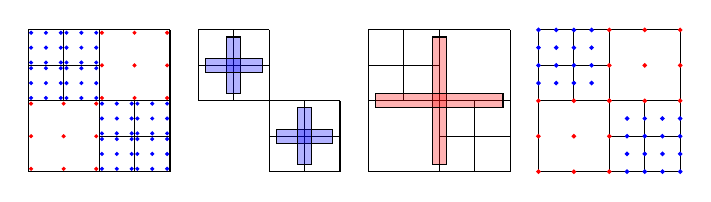
\begin{tikzpicture}[scale=0.18,every node/.style={scale=0.6}]
		
		\begin{scope}[shift={(0,0)}]
		\draw[step=5] (0,0) grid +(10,10);
		\draw[step=2.5] (5,0) grid +(5,5);
		\draw[step=2.5] (0,5) grid +(5,5);
		%\draw[fill=red,fill opacity=0.3] (4.5,0.5) rectangle +(1,9);
		%\draw[fill=red,fill opacity=0.3] (0.5,4.5) rectangle +(9,1);
		%\draw[fill=blue,fill opacity=0.3] (2.0,5.5) rectangle +(1,4);
		%\draw[fill=blue,fill opacity=0.3] (0.5,7.0) rectangle +(4,1);
		%\draw[fill=blue,fill opacity=0.3] (5.5,2.0) rectangle +(4,1);
		%\draw[fill=blue,fill opacity=0.3] (7.0,0.5) rectangle +(1,4);
		%\draw[fill=red!60] (4.2,4.2) circle (0.15);
		
		\def \r{0.1}
		\foreach \x in {0.2,2.5,4.8}{
			\foreach \y in {0.2,2.5,4.8}{
				\draw[red,fill=red] (\x,\y) circle (\r);
			}
		}
		
		\foreach \x in {5.2,7.5,9.8}{
			\foreach \y in {5.2,7.5,9.8}{
				\draw[red,fill=red] (\x,\y) circle (\r);
			}
		}	
		
		\foreach \x in {0.2,1.25,2.3,2.7,3.75,4.8}{
			\foreach \y in {5.2,6.25,7.3}{
				\draw[blue,fill=blue] (\x,\y) circle (\r);
			}
			\foreach \y in {7.7,8.75,9.8}{
				\draw[blue,fill=blue] (\x,\y) circle (\r);
			}  
		}
		
		\foreach \x in {5.2,6.25,7.3,7.7,8.75,9.8}{
			\foreach \y in {0.2,1.25,2.3}{
				\draw[blue,fill=blue] (\x,\y) circle (\r);
			}
			\foreach \y in {2.7,3.75,4.8}{
				\draw[blue,fill=blue] (\x,\y) circle (\r);
			}  
		}
		\end{scope}
		
		\begin{scope}[shift={(12,0)}]
		%\draw[step=5] (0,0) grid +(10,10);
		\draw[step=2.5] (5,0) grid +(5,5);
		\draw[step=2.5] (0,5) grid +(5,5);
		\draw[-] (0,5) -- (5,5);
		\draw[-] (5,0) -- (5,5);
		%\draw[fill=red,fill opacity=0.3] (4.5,0.5) rectangle +(1,9);
		%\draw[fill=red,fill opacity=0.3] (0.5,4.5) rectangle +(9,1);
		\draw[fill=blue,fill opacity=0.3] (2.0,5.5) rectangle +(1,4);
		\draw[fill=blue,fill opacity=0.3] (0.5,7.0) rectangle +(4,1);
		\draw[fill=blue,fill opacity=0.3] (5.5,2.0) rectangle +(4,1);
		\draw[fill=blue,fill opacity=0.3] (7.0,0.5) rectangle +(1,4);
		%\draw[fill=red!60] (4.2,4.2) circle (0.15);
		\end{scope}
		
		
		\begin{scope}[shift={(24,0)}]
		\draw[step=5] (0,0) grid +(10,10);
		\draw[step=2.5] (5,0) grid +(5,5);
		\draw[step=2.5] (0,5) grid +(5,5);
		\draw[fill=red,fill opacity=0.3] (4.5,0.5) rectangle +(1,9);
		\draw[fill=red,fill opacity=0.3] (0.5,4.5) rectangle +(9,1);
		%\draw[fill=blue,fill opacity=0.3] (2.0,5.5) rectangle +(1,4);
		%\draw[fill=blue,fill opacity=0.3] (0.5,7.0) rectangle +(4,1);
		%\draw[fill=blue,fill opacity=0.3] (5.5,2.0) rectangle +(4,1);
		%\draw[fill=blue,fill opacity=0.3] (7.0,0.5) rectangle +(1,4);
		%\draw[fill=red!60] (4.2,4.2) circle (0.15);
		\end{scope}
		
		\begin{scope}[shift={(36,0)}]
        
        \draw[step=5] (0,0) grid +(10,10);
		\draw[step=2.5] (5,0) grid +(5,5);
		\draw[step=2.5] (0,5) grid +(5,5);
		
		\def \r{0.12}
		\foreach \x in {0,2.5,5}{
			\foreach \y in {0,2.5,5}{
				\draw[red,fill=red] (\x,\y) circle (\r);
			}
		}
		
		\foreach \x in {5,7.5,10}{
			\foreach \y in {5,7.5,10}{
				\draw[red,fill=red] (\x,\y) circle (\r);
			}
		}
		
		\foreach \x in {0,1.25,2.5,3.75}{
			\foreach \y in {6.25,7.5,8.75,10}{
				\draw[blue,fill=blue] (\x,\y) circle (\r);
			}
		}	
		
		\foreach \x in {6.25,7.5,8.75,10}{
			\foreach \y in {0,1.25,2.5,3.75}{
				\draw[blue,fill=blue] (\x,\y) circle (\r);
			}
		}
		\end{scope}
		\end{tikzpicture}
		\caption{A simple example of how the cell nodes are placed for quadratic elements in a quadtree. The leftmost figure shows the \textit{locally shared nodes}, which contain duplicates that need to be resolved in order to get \textit{unique shared nodes} (the rightmost figure). We perform a single bottom-up pass of the tree resolving node conflicts, at the corresponding interior region indicated by the same color. 
		\label{fig:cgnodes}}
\end{figure}

\subsection{Efficient SFC-based $kD$-tree traversal}
\label{subsec:treetraverse}
In this section, we present an extension of \tsort~ algorithm to perform efficient traversals on $kD$ trees in order to perform FEM computations. The state-of-the-art approaches\cite{Dendro, mantle, BADER2005994, SundarSampathBiros08} use lookup-tables such as element-to-node mappings, to perform matrix/vector assembly and \mvec. 
%The major drawbacks of these neighborhood data structures include, increasing computational complexity \& memory footprint for higher dimensions and indirect memory accesses lead to bad performances in heterogeneous clusters with deep memory hierarchies. 
In this section, we describe the top-down and bottom-up traversal of the $kD$-tree that are needed for performing these operations without the use of any lookup-tables.
% traversals, which can be top-down, bottom-up or combinations of above, can be used to perform numerical computations which require elemental local nodal values such as FEM computations. 

\textbf{top-down}: In top-down tree traversal for a given non-leaf node $e$, at the corresponding node coordinates, we perform bucketing of the coordinates to the children of $e$, with duplication for the coordinates shared across multiple children (see Figure \ref{fig:traversal}). This process is repeated recursively until we reach a leaf node which can be detected based on the number of coordinates in the bucket. Some buckets might have fewer than the prescribed number of nodes for an element of the specified order. This is because of hanging nodes, and since the nodes of the parent are available at this level, we interpolate these missing values. We recurse in a depth-first fashion as that exposes memory locality and is better suited for deep-memory hierarchies. %Due to the adaptive nature of the tree when we reach a leaf node, some coordinates might be hanging, and those nodal should be able to interpolate from the immediate parent node, due to 2:1 balancing. 

\textbf{bottom-up}: Once we reach a leaf node, we can perform elemental operations ({\em e.g.} elemental \mvec), and if the computation requires an accumulation, nodal values are merged in the reverse direction of the duplication in top-down approach (see \ref{fig:traversal}). 

 \begin{figure}[hbt]
  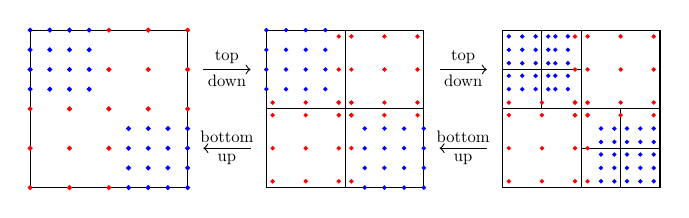
\begin{tikzpicture}[scale=0.2,every node/.style={scale=0.6} ]
	\tikzstyle{edge from parent}=[black,->,shorten <=1pt,>=stealth',semithick,draw]
	\tikzstyle{level 1}=[sibling distance=8mm]
	\tikzstyle{level 2}=[sibling distance=6mm]
	\tikzstyle{level 3}=[sibling distance=4mm]
		
		\begin{scope}[shift={(0,0)}]
		\draw[step=10] (0,0) grid +(10,10);
		%\draw[step=2.5] (5,0) grid +(5,5);
		%\draw[step=2.5] (0,5) grid +(5,5);
		\def \r{0.12}
		\foreach \x in {0,2.5,5}{
			\foreach \y in {0,2.5,5}{
				\draw[red,fill=red] (\x,\y) circle (\r);
			}
		}
		\foreach \x in {5,7.5,10}{
			\foreach \y in {5,7.5,10}{
				\draw[red,fill=red] (\x,\y) circle (\r);
			}
		}
		\foreach \x in {0,1.25,2.5,3.75}{
			\foreach \y in {6.25,7.5,8.75,10}{
				\draw[blue,fill=blue] (\x,\y) circle (\r);
			}
		}	
		\foreach \x in {6.25,7.5,8.75,10}{
			\foreach \y in {0,1.25,2.5,3.75}{
				\draw[blue,fill=blue] (\x,\y) circle (\r);
			}
		}
		\end{scope}
		
		\begin{scope}[shift={(15,0)}]
		\draw[step=5] (0,0) grid +(10,10);
		%\draw[step=2.5] (5,0) grid +(5,5);
		%\draw[step=2.5] (0,5) grid +(5,5);
		\def \r{0.1}
		\foreach \x in {0.4,2.5,4.6,5.4}{
			\foreach \y in {0.4,2.5,4.6,5.4}{
				\draw[red,fill=red] (\x,\y) circle (\r);
			}
		}
		\foreach \x in {4.6,5.4,7.5,9.6}{
			\foreach \y in {4.6,5.4,7.5,9.6}{
				\draw[red,fill=red] (\x,\y) circle (\r);
			}
		}
		\foreach \x in {0,1.25,2.5,3.75}{
			\foreach \y in {6.25,7.5,8.75,10}{
				\draw[blue,fill=blue] (\x,\y) circle (\r);
			}
		}	
		\foreach \x in {6.25,7.5,8.75,10}{
			\foreach \y in {0,1.25,2.5,3.75}{
				\draw[blue,fill=blue] (\x,\y) circle (\r);
			}
		}
		\end{scope}
		
		\begin{scope}[shift={(30,0)}]
		\draw[step=5] (0,0) grid +(10,10);
	    \draw[step=2.5] (5,0) grid +(5,5);
		\draw[step=2.5] (0,5) grid +(5,5);
		\def \r{0.1}
		
		\foreach \x in {0.4,2.5,4.6,5.4}{
			\foreach \y in {0.4,2.5,4.6,5.4}{
				\draw[red,fill=red] (\x,\y) circle (\r);
			}
		}
		\foreach \x in {4.6,5.4,7.5,9.6}{
			\foreach \y in {4.6,5.4,7.5,9.6}{
				\draw[red,fill=red] (\x,\y) circle (\r);
			}
		}
		
		\foreach \x in {0.4,1.25,2.1,2.9,3.35,4.15}{
			\foreach \y in {6.25,7.1,7.9,8.75,9.6}{
				\draw[blue,fill=blue] (\x,\y) circle (\r);
			}
		}	
		\foreach \x in {6.25,7.1,7.9,8.75,9.6}{
			\foreach \y in {0.4,1.25,2.1,2.9,3.75}{
				\draw[blue,fill=blue] (\x,\y) circle (\r);
			}
		}
		
		\end{scope}
		\draw[->] (11,7.5) -- node[above] {top} node[below] {down} (14,7.5);
		\draw[->] (14,2.5) -- node[above] {bottom} node[below] {up} (11,2.5);	
		
		\draw[->] (26,7.5) -- node[above] {top} node[below] {down} (29,7.5);
		\draw[->] (29,2.5) -- node[above] {bottom} node[below] {up} (26,2.5);	
		
		\end{tikzpicture} 
		%\vfill
		
		\begin{tikzpicture}[scale=1.2, level distance=8mm,emph/.style={edge from parent/.style={red,->,shorten <=1pt,>=stealth',very thick,draw}},norm/.style={edge from parent/.style={black,->,shorten <=1pt,>=stealth',semithick,draw}}]
    	\tikzstyle{edge from parent}=[black,->,shorten <=1pt,>=stealth',semithick,draw]
    	\tikzstyle{level 1}=[sibling distance=8mm]
    	\tikzstyle{level 2}=[sibling distance=6mm]
    	\tikzstyle{level 3}=[sibling distance=4mm]
    	
    	\node[fill=red!30,rounded corners] {root}
    	child[emph] { node[fill=blue!30,rounded corners] {nl}
    		child[norm] { node[fill=green!30,rounded corners] {a}}
    		child[emph] { node[fill=green!30,rounded corners] {b}
    			%child[norm] { node[fill=green!30,rounded corners] {b}}
    			%child[norm] { node[fill=green!30,rounded corners] {c}}
    			%child[emph] { node[draw=red,very thick,fill=green!30,rounded corners] {d}}
    			%child[norm] { node[fill=green!30,rounded corners] {e}}
    		}
    		child[norm] { node[fill=green!30,rounded corners] {f}}
    		child[norm] { node[fill=green!30,rounded corners] {g}}
    	}
    	child { node[fill=green!30,rounded corners] {h}}
    	child { node[fill=green!30,rounded corners] {i}}
    	child { node[fill=blue!30,rounded corners] {nl}
    		child { node[fill=green!30,rounded corners] {j}}
    		child { node[fill=green!30,rounded corners] {k}}
    		child { node[fill=green!30,rounded corners] {l}}
    		child { node[fill=green!30,rounded corners] {m}}
    	};
    	
    	%% Draw levels axis ...
    	\draw[->] (-3,0) -- (-3,-2);		
    	\draw[snake=ticks,segment length=0.95cm] (-3,0) -- (-3,-2);
    	
    	\draw (-2.8,0) node {$0$}
    	(-2.8,-0.8) node {$1$}
    	(-2.8,-1.6) node {$2$};
    	%(-2.8,-2.4) node {$3$};
    	\draw (-3.3,-1.6) node [rotate=90] {$level$};		
    	%\draw (3,-2.9) node {$\mathcal{R}$};
	
	    \end{tikzpicture}
		
	\caption{Illustration of top-down \& bottom-up tree traversals for a $2D$ tree with quadratic element order. The leftmost figure depicts the unique shared nodes (nodes are color-coded based on level), as we perform top-down traversal nodes shared across children of the parent get duplicated for each bucket recursively, once leaf node is reached it might be missing elemental local nodes, which can be interpolated from immediate parent (see the rightmost figure). After elemental local node computations, bottom-up traversal performed while merging the nodes duplicated in during the top-down traversal.
	    \label{fig:traversal}
	}
\end{figure}

\begin{figure}
    \centering
    \begin{tikzpicture}
        \draw[thick](2,2,0)--(0,2,0)--(0,2,2)--(2,2,2)--(2,2,0)--(2,0,0)--(2,0,2)--(0,0,2)--(0,2,2);
        \draw[thick](2,2,2)--(2,0,2);
        \draw[gray](2,0,0)--(0,0,0)--(0,2,0);
        \draw[gray](0,0,0)--(0,0,2);
        \draw(1,1,2) node{$t_0$};
        \begin{scope}[shift={(4,0)}]
        \draw[thick](2,2,0)--(0,2,0)--(0,2,2)--(2,2,2)--(2,2,0)--(2,0,0)--(2,0,2)--(0,0,2)--(0,2,2);
        \draw[thick](2,2,2)--(2,0,2);
        \draw[gray](2,0,0)--(0,0,0)--(0,2,0);
        \draw[gray](0,0,0)--(0,0,2);
        \draw(1,1,2) node{$t_1$};
        \end{scope}
        
        \draw[thick,dotted] (2,0,2) to[out=-20,in=-70] (6,0,2);
        \draw[thick,dotted] (0,0,2) to[out=-20,in=-70] (4,0,2);
        
        \draw[gray,dotted] (0,0,0) to[out=-20,in=-70] (4,0,0);
        \draw[gray,dotted] (2,0,0) to[out=-20,in=-70] (6,0,0);
        
        \draw[gray,dotted] (2,2,0) to[out=60,in=120] (6,2,0);
        \draw[gray,dotted] (0,2,0) to[out=60,in=120] (4,2,0);
        
        \draw[thick,dotted] (2,2,2) to[out=60,in=120] (6,2,2);
        \draw[thick,dotted] (0,2,2) to[out=60,in=120] (4,2,2);
        
        \draw[thick, -latex'] (2,3,0) -- (4,3,0) node[above] {$time$};
        
    \end{tikzpicture}
    \caption{Illustration of a \stra. A simple interpretation is that of an octant (in space) represented at two time points, $t_0$ and $t_1$. \label{fig:sedecant}}
\end{figure}

\subsection{Matrix-free implementation on $4D$ meshes}
\label{s:mvec}

As mentioned in the previous section, we will only store the $4D$ coordinates and not any maps (such as element-to-node maps). There are two major reasons for this. Firstly, these maps are very expensive to construct and will have a large memory footprint for $4D$ meshes. Secondly, the variables of interest are accessed and updated using such maps during FEM computations and as such amount to indirect memory access. For large $4D$ meshes in particular, such indirect memory access is likely to be extremely inefficient on modern architectures with high levels of parallelism and deep memory hierarchies. To this effect, we propose a {\em mesh-free} approach that makes use of the quasi-structured nature of \stri s and enables direct access to data. We explain this approach in detail and provide evidence for the efficacy of this approach.  

%For clarity of presentation, we use a simple system system, say corresponding to the heat equation, to explain the $4d$ \mvec. 
We will illustrate a \mvec\ with the transient diffusion operator ($\frac{\partial}{\partial t} + \nabla^2$), given in a discrete form as $K$, i.e., we will compute $v=K u$. Here $u$ is the scalar unknown defined over our spacetime domain, i.e., there is one unknown per node (coordinate point). Therefore the input to our \mvec\ will be the \texttt{real} vector $u$ and another vector of points $\mathbf{p}=(x,y,z,t)$ ($4\times$ \texttt{unsigned int}). The output will be the vector $v$, the same size as $u$ such that $v=K u$. Unlike conventional FEM codes, we will evaluate $v$ without requiring indirect memory accesses to $u,v$ or $\mathbf{p}$. Note that our approach becomes significantly more effective for systems with multiple dofs per spatio-temporal point, as these all will use the same coordinate information. This will be especially useful for both the Navier-Stokes equations (with 4 dofs per point), and the Poisson-Nerst-Plank equations ($n_s+1$ dofs per point, where $n_s$ is the number of species considered).

Since we do not have a mesh, we will have to extract the required information on the fly. Similar to the \stri\ construction, (Figure~\ref{fig:cons}), we proceed in a top-down fashion using the radix sort. This is particularly efficient since we have the $x,y,z$ and $t$ coordinates as \texttt{unsigned int}s. Also, since the coordinates and the unknowns are arranged using space filling curves, there is high locality. In MSD radix, we use the bits--from most to least significant--to bucket the data. In our case, at each level we use one bit each from the $x,y,z$ and $t$ coordinates to bucket the points ($\mathbf{p}$) and unknowns $u$. We then recurse within each bucket. This happens in a depth-first fashion that in combination with the locality of space filling curves, make the overall data-access amenable to modern deep memory hierarchies. Bucketing within radix sort involves only direct memory in a streaming fashion and requires one cache-line for accessing the input and one each for each bucket. 
%Based on the architecture, one can decide to bucket two levels simultaneously ($64$ buckets) using $2$ bits each from $x,y$ and $z$.

\begin{figure}

	 \begin{minted}[frame=lines]{python}
v = {0} 
n = num_non_zero_basis_per_element		
nb = num_buckets;

def matvec(u, x, v, l): # compute v = Ku 
 (U, X, V) = scatter_to_buckets(u, x, v, l)
 for (ui, xi, vi) in (U, X, V):
   if len(xi) == n: # leaf
     for i in [0,n):
       for j in [0,n):
         vi[j] += K_e[i,j] * ui[i];
   else:
     matvec(ui, xi, vi, l-1) # recurse

   gather_from_buckets(vi, x, v, l) 

def U,X = scatter_to_buckets(u, x, l):
 cnt = zeros[nb+1] 
 for _x in x: 
   cnt[_x & (1 << l) + 1]++  
 for (_u, _x) in (u, x):  
   idx = cnt[_x & (1<<l)]++
   U[idx] = _u  
	 X[idx] = _x

def gather_from_buckets(u, x, v, l):
  ... 
  for i in [0,len(x)):  
    idx = cnt[x[i] & (1<<l)]++
    v[i] += u[idx]    
		\end{minted}	
% 	\end{minipage}
	\caption{\label{fig:matvec} \small The pseudocode for the mesh-free $4D$ FEM \texttt{matvec}. Here we compute $v = Ku$ where $u,v$ are specified at coordinates $x,~t$ and $l$ is the level of the \stri, typically $30$. Note that the recursion can terminate early on hitting a leaf node. 
	Note that while access might appear indirect within \texttt{scatter\_to\_bucket} and \texttt{gather\_from\_buckets}, these indices are the bucket numbers and typically small, and $u$ and $v$ are still accessed sequentially, as \texttt{idx} is incremented. 
	While the mesh-free code appears complex, in preliminary tests, %(see Table~\ref{tab:results}), 
	it is approximately $5\times$ faster for scalar PDEs, with the speedup
	increasing for problems with larger dofs.
	}
\end{figure}

Bucketing for the \mvec\ is a bit more involved, so we first illustrate in $2D$ in Figure~\ref{fig:traversal}. Here we need to bucket the interior points and replicate the interior shared faces and the interior corner as well. In $4D$, %Since we bucket recursively, it is sufficient to consider the bucketing from one \stra\ to its children. 
we need to bucket the volumes (faces in 3D) and the interior faces, edges and volumes as these dofs need to be replicated across octants. Once replicated, the \stra s are independent of each other and can recurse independently. This expresses a very fine-grained parallelism not possible with traditional FEM \mvec s. As previously explained, we identify reaching the leaf node based on the when all dofs correspond to the nodes of a single element, potentially with interpolation in case of hanging nodes. Having reached the leaf node, we apply the elemental operator %\footnote{We skip details as either a precomputed elemental matrix or numerical quadrature can be performed and does not affect overall scalability or performance.} 
to compute $v_e = K_e u_e$. On the return, the results in $v$ are accumulated from all children. This is the opposite of the duplication of $u$ prior to the recursion. The simplified pseudocode for the \mvec\ is presented in Figure~\ref{fig:matvec}. 
%For clarity of presentation, we have skipped data-interpolations that are needed by both the traditional as well as mesh-free approaches while working with adaptively refined meshes, such as octrees or \stri s. This does not affect any of the algorithms, and interpolations in both cases happen from parent to child, only when we reach a leaf node. 
%While we have used the recursive formulation for clarity of presentation, the actual implementation uses an iterative variant as that is more efficient. \mf{Is this correct?}

%\hs{data-first, no indirect, fine-grained parallelism.} 
The mesh-free \mvec\ approaches the computation in a data-first fashion and is structured based on the data dependencies and the associated data movement. Note that in the distributed memory setting, we follow a similar principle and exchange ghost or halo regions, albeit using additional lookup tables. Since the mesh-free approach exposes such parallelism in a hierarchical fashion (due to the tree structure), the same basic algorithm holds for the distributed memory cases as well, except that the bucketing at the inter-process level will require {\textsc MPI} communication. Again, unlike traditional codes, this can be done without any additional lookup tables (scatter maps). Also note that the resulting code does not have any indirect memory accesses to the large data arrays $u$ and $v$. This makes implementations simple and easy enough for modern compilers to optimize (such as prefetching, vectorization, etc.) without special architecture specific tuning of the code. 
